% !TEX TS-program = pdflatex
% !TEX encoding = UTF-8 Unicode

\documentclass[11pt]{article} % use larger type; default would be 10pt

\usepackage[utf8]{inputenc} % set input encoding (not needed with XeLaTeX)

\usepackage{geometry} % to change the page dimensions
\geometry{a4paper} % or letterpaper (US) or a5paper or....
\usepackage{graphicx} % support the \includegraphics command and options

%%% PACKAGES
\usepackage{booktabs} % for much better looking tables
\usepackage{array} % for better arrays (eg matrices) in maths
\usepackage{paralist} % very flexible & customisable lists (eg. enumerate/itemize, etc.)
\usepackage{verbatim} % adds environment for commenting out blocks of text & for better verbatim
\usepackage{subfig} % make it possible to include more than one captioned figure/table in a single float
\usepackage{minted} % Code syntax highlighting
\usepackage[x11names,table]{xcolor}
\usepackage[]{caption}
\captionsetup{justification=raggedright,singlelinecheck=false,labelsep=newline,labelfont=bf,textfont=it}
\usepackage[parfill]{parskip}
\usepackage[textsize=tiny]{todonotes}
\usepackage{tikz}
\usepackage{lmodern}

\newcommand\code[2][]{
    \tikz[baseline=(s.base)]{
        \node(s)[
            rounded corners,
            fill=gray!20,        % background color
            draw=gray,          % border of box
            text=gray!50!black, % text color
            inner xsep =3pt,    % horizontal space between text and border
            inner ysep =0pt,    % vertical space between text and border
            text height=2ex,    % height of box
            text depth =1ex,    % depth of box
            #1                  % other options
        ]{\texttt{#2}};
    }
}

\DeclareCaptionFont{blue}{\color{black}}
\newcommand{\maketimelinepart}{\color{black}\makebox[0pt]{\textbullet}\hskip-0.5pt\vrule width 1pt\hspace{\labelsep}}

\usepackage{sansmathfonts}
\usepackage[T1]{fontenc}
\renewcommand*\familydefault{\sfdefault}

\usepackage[%
  style = apa,
  sortcites = true, 
  sorting = nyt, 
  backend = biber]{biblatex}
\bibliography{biblio.bib}

%%% HEADERS & FOOTERS
\usepackage{fancyhdr} % This should be set AFTER setting up the page geometry
\pagestyle{fancy} % options: empty , plain , fancy
\renewcommand{\headrulewidth}{0pt} % customise the layout...
\lhead{}\chead{}\rhead{}
\lfoot{}\cfoot{Page \textbf{\thepage}}\rfoot{}

\usepackage[pdftex,
            pdfauthor={up2193347},
            pdftitle={MEGA Report},
            pdfsubject={Implementing a Maths Library and Basic Physics Engine in C++},
            pdfkeywords={maths, mega, physics}]{hyperref}
\hypersetup{
    hidelinks
}

% Prevent hyphenation of words.
\righthyphenmin=5
\lefthyphenmin=5

%%% ToC (table of contents) APPEARANCE
\usepackage[nottoc,notlof,notlot]{tocbibind} % Put the bibliography in the ToC
\usepackage[titles,subfigure]{tocloft} % Alter the style of the Table of Contents
\renewcommand{\cftsecfont}{\sffamily\bfseries\upshape}
\renewcommand{\cftsecpagefont}{\sffamily\mdseries\upshape} % No bold!

%%% END Article customizations

%%% The "real" document content comes below...

\title{Maths For Games\\Report}
\author{up2193347}
%\date{} % Activate to display a given date or no date (if empty),
         % otherwise the current date is printed 

\begin{document}

\maketitle
\tableofcontents
\pagebreak

\section{Artefact Overview}

For this assignment, I implemented a basic 3D physics engine based on \textit{Game Physics In One Weekend} \autocite{hodges_game_2021}, 
and an accompanying OpenGL renderer.

A 30 second video of the artefact running is viewable here:\\\textcolor{blue}{https://www.youtube.com/watch?v=blah}.

\todo{Add the video}

\subsection{Renderer}

\todo{IMAGES!!}

I created a basic OpenGL renderer capable of rendering 3D meshes, quads, and text.
This required the implementation of projection and transformation matrices, the understanding of the representation
of 3D meshes as vertices, normal vectors, and indices, and a basic lighting function.

\subsection{Physics Engine}

I created a custom physics engine based on \textit{Game Physics In One Weekend} \autocite{hodges_game_2021}. It 
features sphere bodies that can collide realistically, and a codebase that can be extended to add further
body types. The physics engine is integrated with the renderer to visualise the physics simulation, and provide
an interface to add and remove objects from the simulation, and adjust the timescale.

\todo{IMAGES!!}

\section{Maths Library}

\subsection{Vectors}

The core of rendering and physics are \textbf{vectors}. When implementing vectors, I templated the backing type, 
such that a vector could be made of floats or doubles without having to copy all of the code. This could be useful
if higher precision is needed, and allows for a compile-time toggle to increase physics accuracy at the cost of 
performance (as doubles take double the space in SIMD registers).

My vector type includes operator overloads and functions for:

\begin{itemize}
  \item Addition, subtraction, multiplication, and division
  \item Length and squared length
  \item Normalisation
  \item Dot products
  \item Cross products
  \item Converting to Euler angles
\end{itemize}

\subsection{Euler Angles \& Quaternions}

I implemented both Euler angles and quaternions. Euler angles are much simpler to work with, as they represent
rotations in a much more natural way, and can be converted to a rotation matrix in less operations.
However, the problem of gimbal lock is much worse in the context of a physics engine, so quaternions are a must.
I still use Euler angles in the renderer, so there are a lot of conversions between Euler and quaternions, 
and degrees and radians. An implementation that is made to only use quaternions may perform faster due to less 
conversions.

\todo{code snippets}

\subsection{Matrices}

Like vectors, my Matrix type is also templated, including the size of the Matrix (although it is limited to 
square matrices). I did this to reduce the amount of lines of code required to implement the types, however
I believe the templating of the Size mainly increased complexity and hurt performance, as 
implementations could be less specialised and involved for loops. I avoided this slightly through the use of \code{if constexpr}, 
which are if statements that are evaluated at compile-time. I also used static asserts to throw errors if 
invalid operations were performed on incorrect sizes, such as initialising a 3x3 matrix with four 4D vectors.
If I were to template matrix sizes again, I would also template vector sizes so vectors could be used as the 
backing type, as the ability to perform cross products (for example) on columns would be useful.

My matrix type has functions for:

\begin{itemize}
  \item Constructing with a scalar in the diagonal
  \item Constructing from vectors
  \item Addition, subtraction, multiplication, and division of matrices
  \item Multiplication of vectors
  \item Transposing
  \item Inverting generally
  \item Finding the determinant
  \item Creating transformation and projection matrices
\end{itemize}

\begin{figure}
  \caption{Code for multiplying 4x4 matrices.}
  \label{mat4x4multiply}
  \centering
  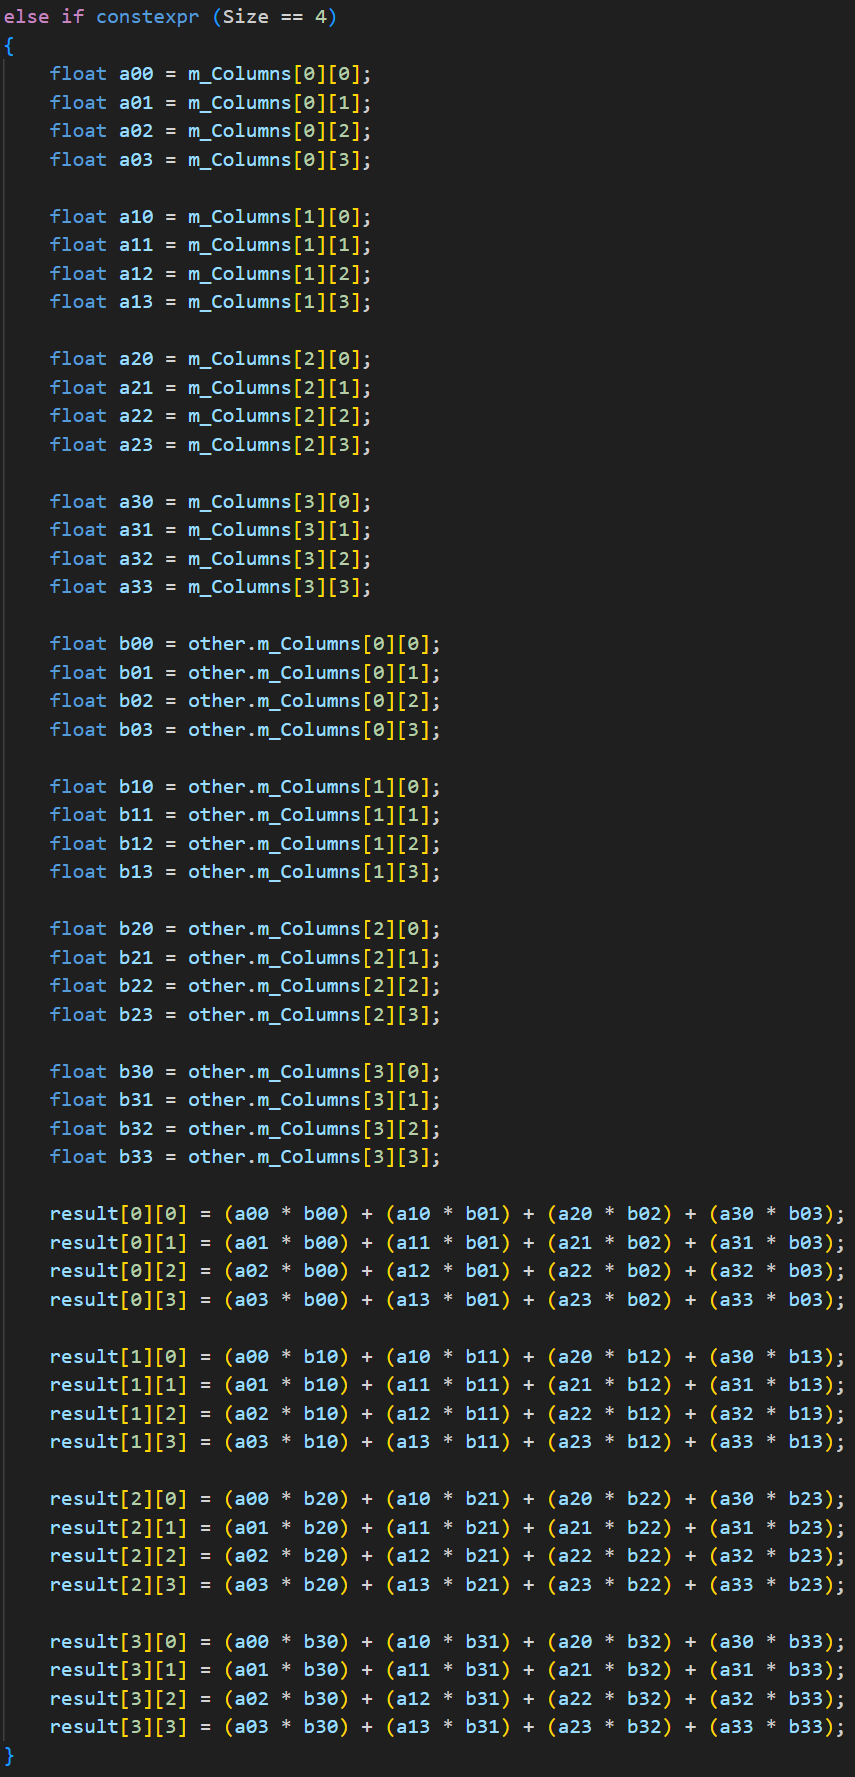
\includegraphics[height=25em]{Images/Mat4Multiplication.png}
  \linebreak
\end{figure}

\begin{figure}
  \caption{Code for finding the transpose of a matrix.}
  \label{mattranspose}
  \centering
  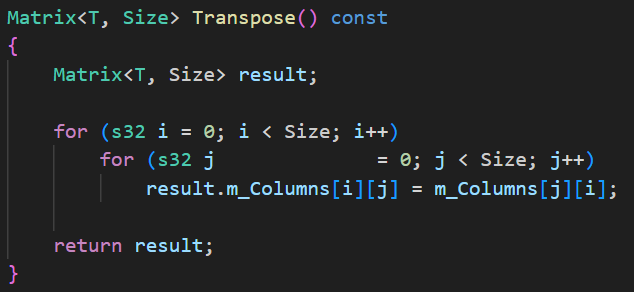
\includegraphics[height=10em]{Images/MatTranspose.png}
  \linebreak
\end{figure}

\todo{code examples}

A consistent issue I encountered with my Matrix class was code that mixed up rows and columns. For example, my 
initial implementation of matrix multiplication had this issue. I debugged this issue mainly through trial and 
error. To avoid this issue in the future, I renamed my data variable from \code{Data} to
\code{Columns}, which made it more explicit in the code that the Matrix data was column-major.

\subsection{Debugging}
\label{debuggingmaths}

When debugging, I used an online matrix calculator \autocite{reshish_inverse_nodate} to validate my results. As seen in Figure
\ref{debuggingmat3invert}, I was able to validate the correctness of my 3x3 inversion function using a calculator, which was 
useful to find in which calculations errors were occurring.

In future, it would perhaps be easier to include an established maths library, such as GLM \autocite{g-truc_creation_glm_2024},
in the codebase such that it could be used as a reference for correct outputs; keeping validation within the code would allow 
the easy use of asserts and the creation of tests. 

\begin{figure}
  \caption{Validating my Matrix 3x3 invert function using an online calculator.}
  \label{debuggingmat3invert}
  \centering
  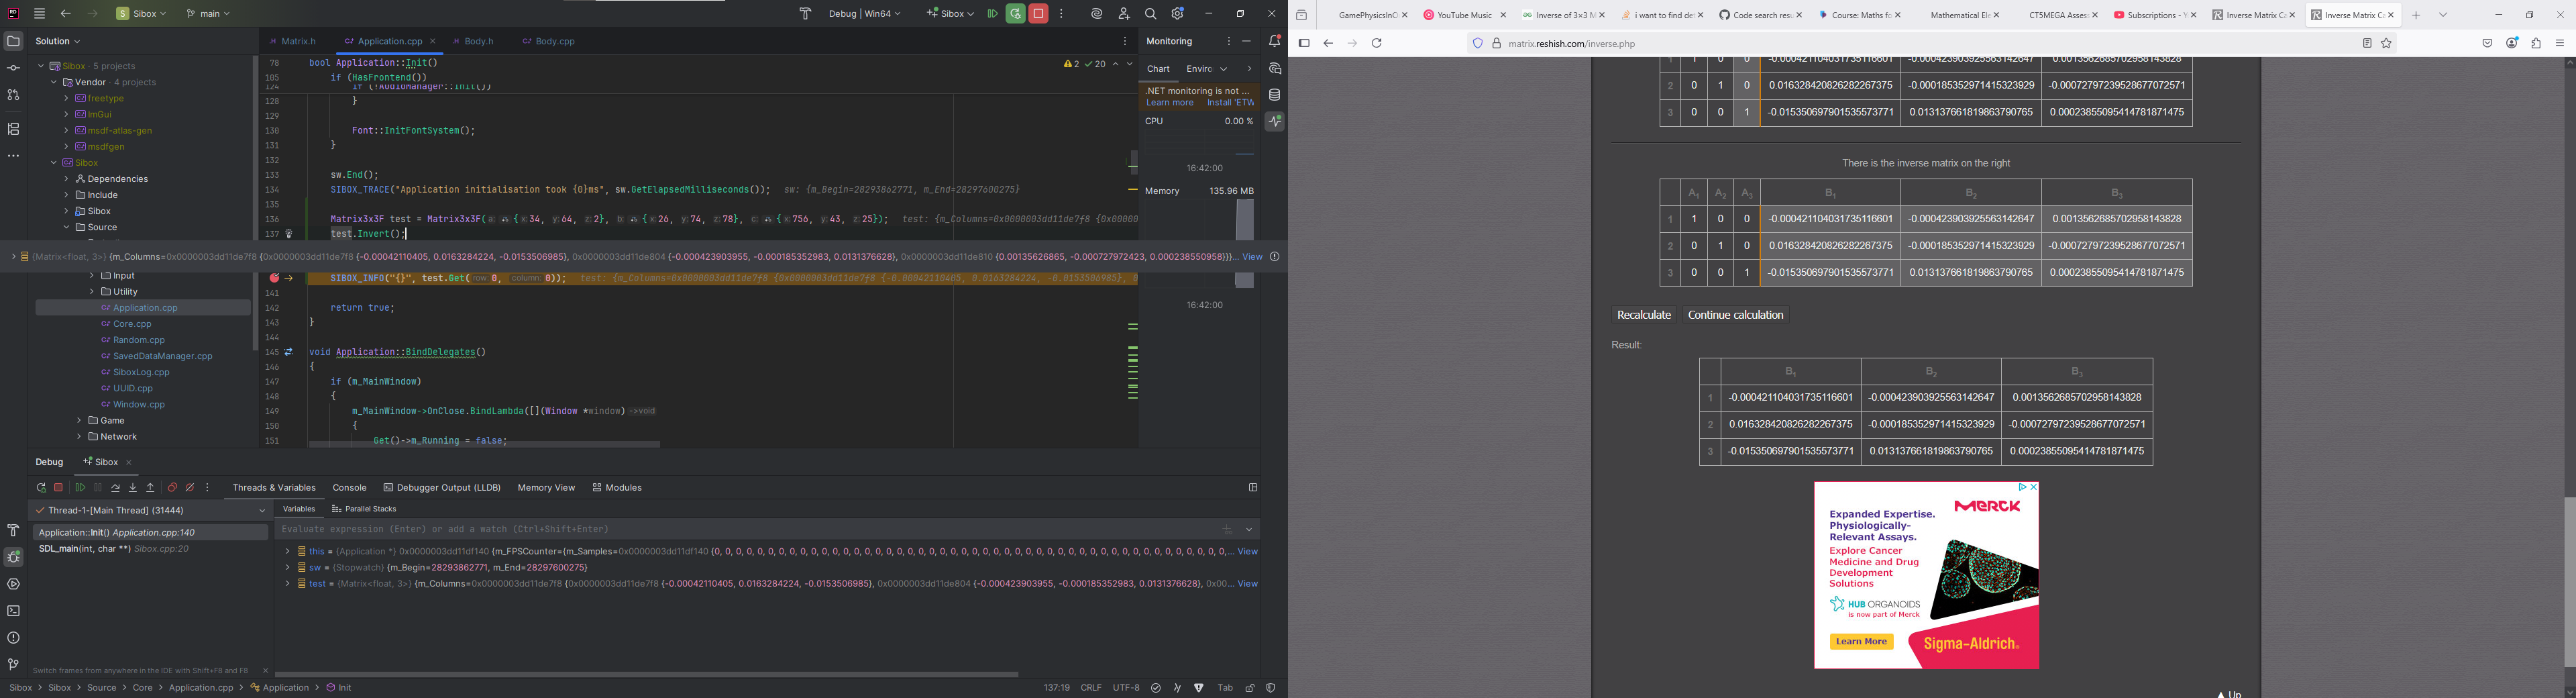
\includegraphics[width=\textwidth]{Images/TestingInverse3x3.png}
  \linebreak
\end{figure}

Debugging was made slightly harder by the use of \code{FORCEINLINE}, as breakpoints can behave unpredictably when
code is inlined. However, inlining was important for performance. A better implementation may have a toggle to
disable \code{FORCEINLINE} in debug builds.

\subsection{General Analysis}

The performance of the library could be improved heavily through the use of SIMD intrinsics, which allow you to 
operate on multiple pieces of data with one CPU instruction. This is mainly for vectors, as matrix multiplication
benefits less from SIMD \autocite{cui_performance_2019}.
However, this complicates the code significantly, so I decided it was out of scope for this project.

\section{3D Renderer}

\subsection{Transformations \& Projections}

Vertex positions must be converted from model space to world space, and then to screen space. Graphics APIs require
vertices to be in the -1 to 1 space, called normalised device coordinates. 

Converting from model space to world space can be done through a transformation matrix. Implementing these were simple,
however I took inspiration from GLM \autocite{g-truc_creation_glm_2024} to optimise the creation of rotation matrices
by merging the individual yaw, pitch, and roll matrices into one matrix creation, as seen in Figure \ref{rotationmatrices}.

To view these world space vertices through a camera and convert to NDC, we need a view-projection matrix. View matrices
are covered by the previous translation matrices. Projections include perspective and orthographic. For a general 3D game,
we need a perspective matrix, which is surprisingly simple to create, as seen in Figure \ref{perspectivematrix}.

\begin{figure}
  \caption{Code for constructing a rotation matrix.}
  \label{rotationmatrices}
  \centering
  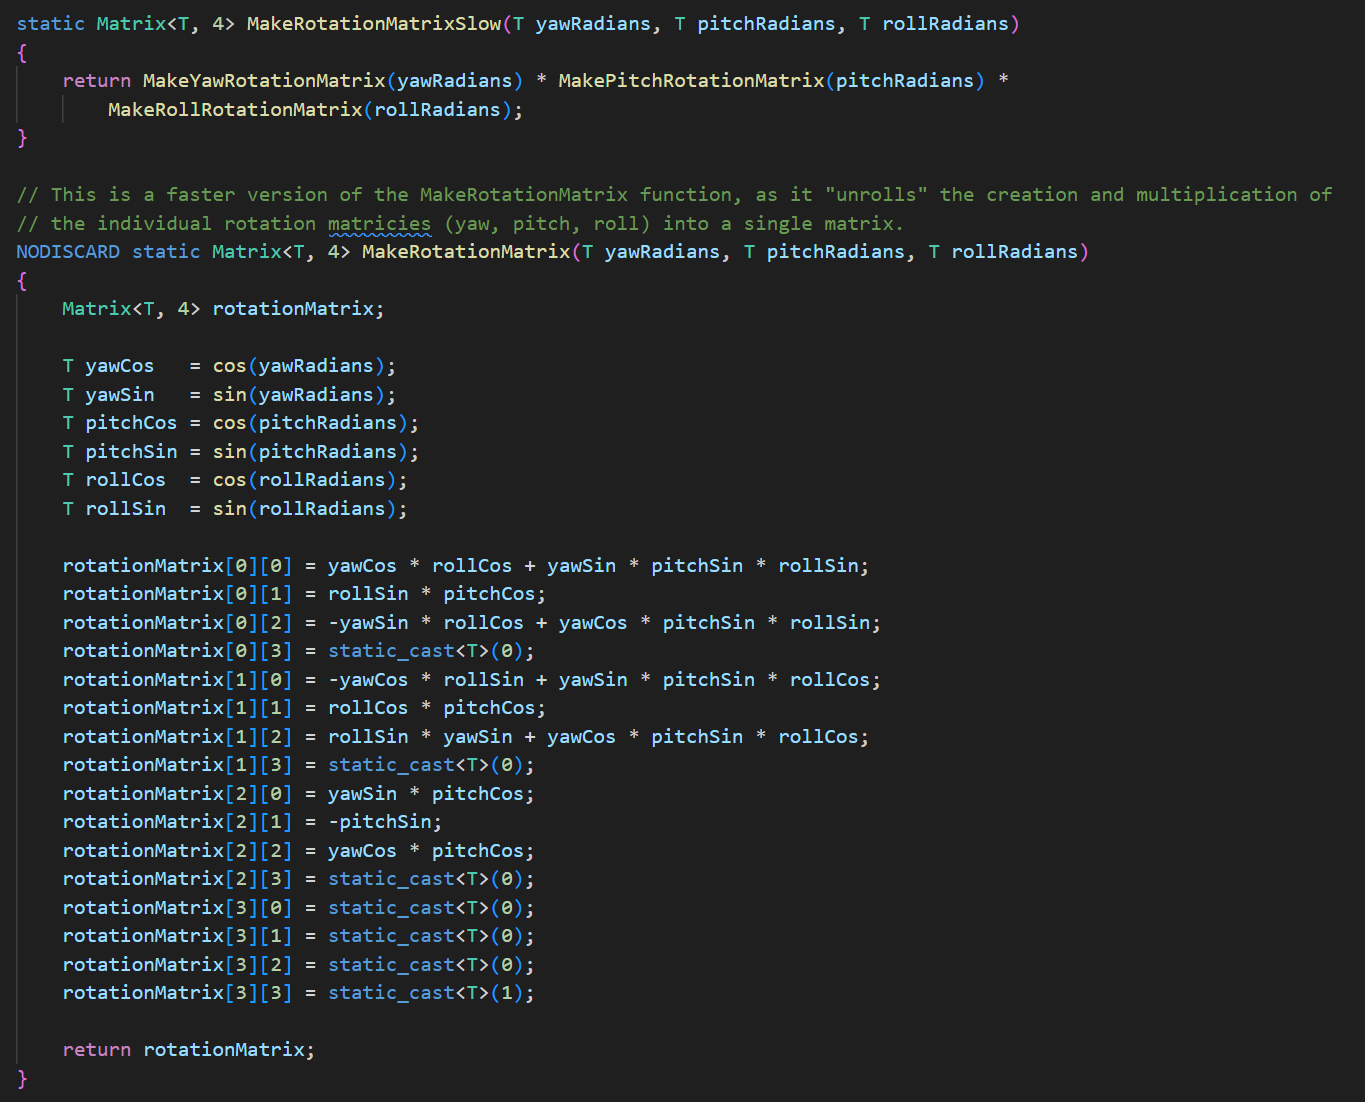
\includegraphics[height=22em]{Images/RotationMatrices.png}
  \linebreak
\end{figure}

\begin{figure}
  \caption{Code for constructing a perspective projection matrix.}
  \label{perspectivematrix}
  \centering
  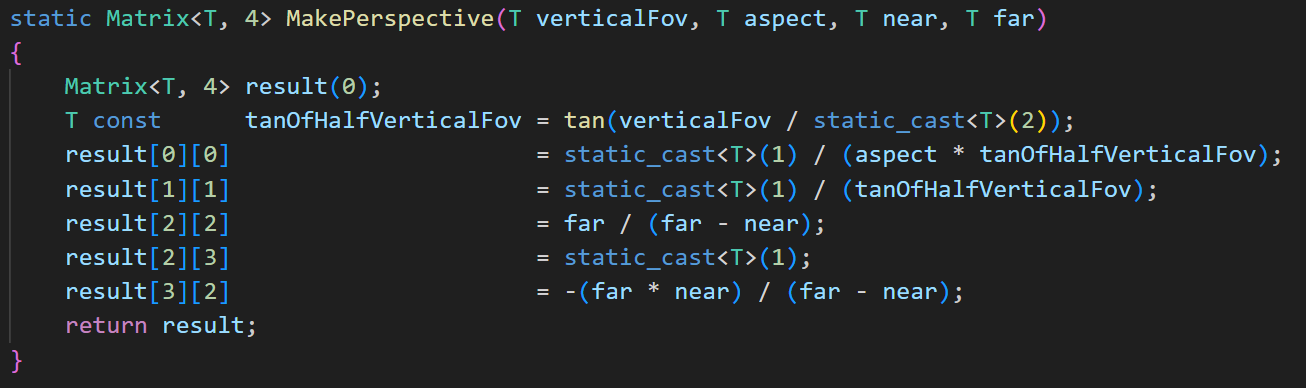
\includegraphics[height=10em]{Images/PerspectiveMat.png}
  \linebreak
\end{figure}

\subsection{Meshes}

Meshes are represented as a list of vertices, all of which have a 3D vector representing their position, a 3D vector for their normal,
and a 2D vector for their texture coordinate. An important point here was ensuring the in-memory layout of my vector classes are correct
such that we can copy the vertex data directly into the arrays, to speed up loading.

\subsubsection{Winding Order}

To determine if a triangle is facing the camera or not, GPUs take the cross product of a triangle's first and second edge \autocite{michel_understanding_2016}.
If that cross product points towards the camera, it's a front face and will be rendered, but if it doesn't, it is discarded.
Therefore, the indices of the mesh determine which way the faces face, as they change which edges are the first and second edges.
I had issues with meshes being inverted, but this was fixed by flipping the indices.

\todo{reword}

\subsection{Lighting}

I implemented basic lighting based on the work of \textcite{phong_illumination_1975}.

\section{Physics Engine}

\todo{Debugging physics. Bodge of multiplying the penetration vector}

\todo{Discuss performance implications of many conversions between units, types.
Rebuild from the top to improve cohesion?}

\todo{Discuss learning notation}

\pagebreak

\section{References}

\setlength{\bibitemsep}{1em}
\printbibliography[heading=none]

\end{document}
